\section{NanoPU Design Overview}
\begin{figure}
  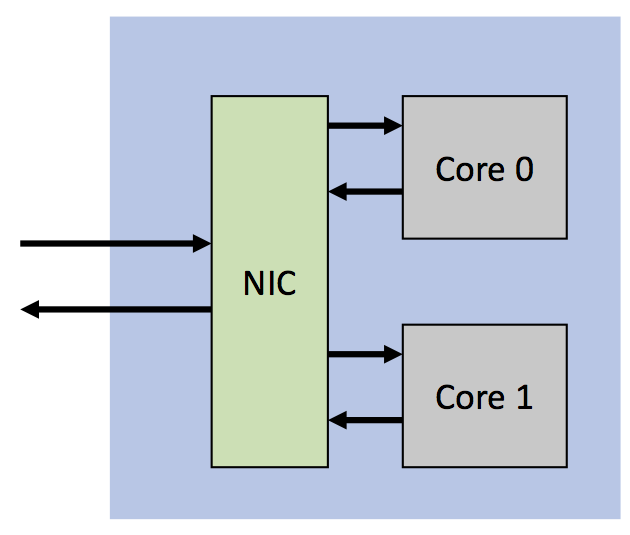
\includegraphics[width=0.75\linewidth]{./figures/NanoPU}
  \caption{High-level NanoPU architecture with 2 cores.}
  \label{fig:NanoPU}
\end{figure}
\begin{itemize}
    \item Domain specific architectures are becoming more and more popular today for good reason.
    \item The slowing of Moore's Law is preventing general purpose compute from getting any faster, so we must turn to domain specific hardware to achieve performance and efficiency gains.
    \item We believe that the domain of compute-intensive distributed applications is in dire need of domain specific hardware.
    \begin{itemize}
        \item General purpose hardware is not optimized to put compute in the network. Instead, it puts memory in the network and attaches compute to memory. \chang{Perhaps we should tell why general-purpose CPUs evolved that way. Is it because the initial designs for CPUs were done when standalone computing (as opposed to distributed computing) was predominant? Or was it because in the early days of CPUs networks were just way too slow (relatively to the speed of the CPUs of those early days), and hence it just didn't make sense to put compute to the network directly?}
        \item General purpose hardware has far too many sources of resource contention which inflate tail latency and kill performance of distributed applications: cache contention, memory bandwidth, CPU cores, and NIC queues. \chang{Isn't dedication or hard partitioning kind of orthogonal to our point? What if someone introduces hard-partitioned cache, memory, memory bandwidth, NIC, etc. for general-purpose CPUs? Sure, it's gonna be expensive, but it may be able to bound the tail latency very well, right? What's wrong with such an architecture for nanoservices?}
    \end{itemize}
    \item We present the NanoPU, which we consider to be a first step towards building a domain-specific processor for compute-intensive distributed applications.
    \item The NanoPU has the following characteristics that make it well suited for the aforementioned domain:
    \begin{itemize}
        \item A fast path from the network to the heart of the CPU core, the register file. This minimizes average communication latency for network communications, drastically improving the common case. This architecture is explicitly designed to scale out beyond a single chip. One of the main goals of the NanoPU is to put as many cores in the network as possible. The NanoPU will allow developers to harness more cores than would ever be possible or practical to fit on a single chip (e.g. millions of cores).
        \item An event-driven PISA pipeline on the NIC which allows it to efficiently terminate a low latency transport protocol like Homa or NDP in hardware. This minimizes the overhead required to send messages because software no longer needs to deal with maintaining timers, sending retransmissions, or reassembling messages because these things can be implemented very efficiently in hardware. We describe the hardware mechanisms within the NanoPU architecture that enable it to terminate a transport protocol in Section XXX.
        \item The NanoPU design introduces the concept of NIC-driven thread scheduling in order to minimize tail latency. The NanoPU's thread scheduling policy enforces strict priority scheduling of nanoserver threads on the core and does not rely on slow software based scheduling mechanisms.
    \end{itemize}
    \item The following sections describe the NIC data-path, the NIC-Core interface, the NanoPU's hardware support for transport protocols, and the NanoPU's minimal operating system (the NanoKernel) in more detail.
\end{itemize}

\subsection{NIC Datapath}
\begin{figure}
  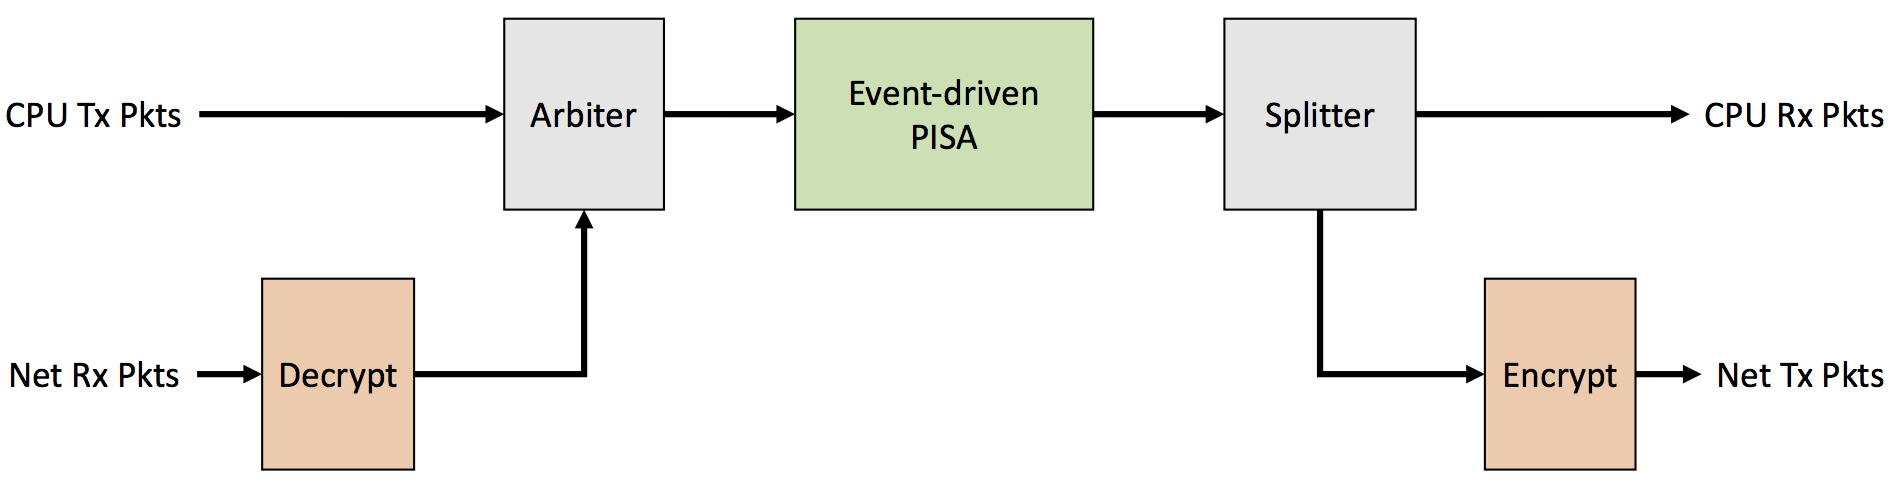
\includegraphics[width=\linewidth]{./figures/NIC-Datapath}
  \caption{High-level NanoPU NIC datapath architecture.}
  \label{fig:NIC-Datapath}
\end{figure}
\begin{itemize}
    \item The NIC Datapath is responsible for processing packets received from both the network and the attached CPU core and forwarding packets either to the network or to the CPU core.
    \item The centerpiece of the NIC datapath is an event-driven PISA pipeline.
    \item Event-driven PISA is a recently proposed programmable packet processing architecture, which supports more expressive stateful data-plane programming than its predecessor: the baseline PISA architecture. Section XXX describes how an event-driven PISA architecture along with additional hardware mechanisms can be used to implement transport protocols in programmable hardware, thus minimizing the overheads required for sending network messages.
    \item In addition to transport processing logic, the PISA pipeline is responsible for adding and removing packet headers as they move between the network and the CPU cores. It removes Ethernet, IP, and L-NIC transport headers, and adds a small application header for packets that arrive from the network and are going to the CPU. It performs the opposite tasks for packets sent from the CPU and are going out the network.
    \item The Event-driven PISA pipeline can also be used to offload some application specific logic in order to improve performance. \chang{what do we mean by this? It sounds vague.}
    \item The data-path also contains a block to decrypt packets as they arrive from the network and a block to encryt packets just before they are sent over the network. This avoids the software overhead that would be incurred if these tasks needed to be performed in the application or the operating system.
\end{itemize}

\subsection{NIC-Core Interface}
\begin{figure}
  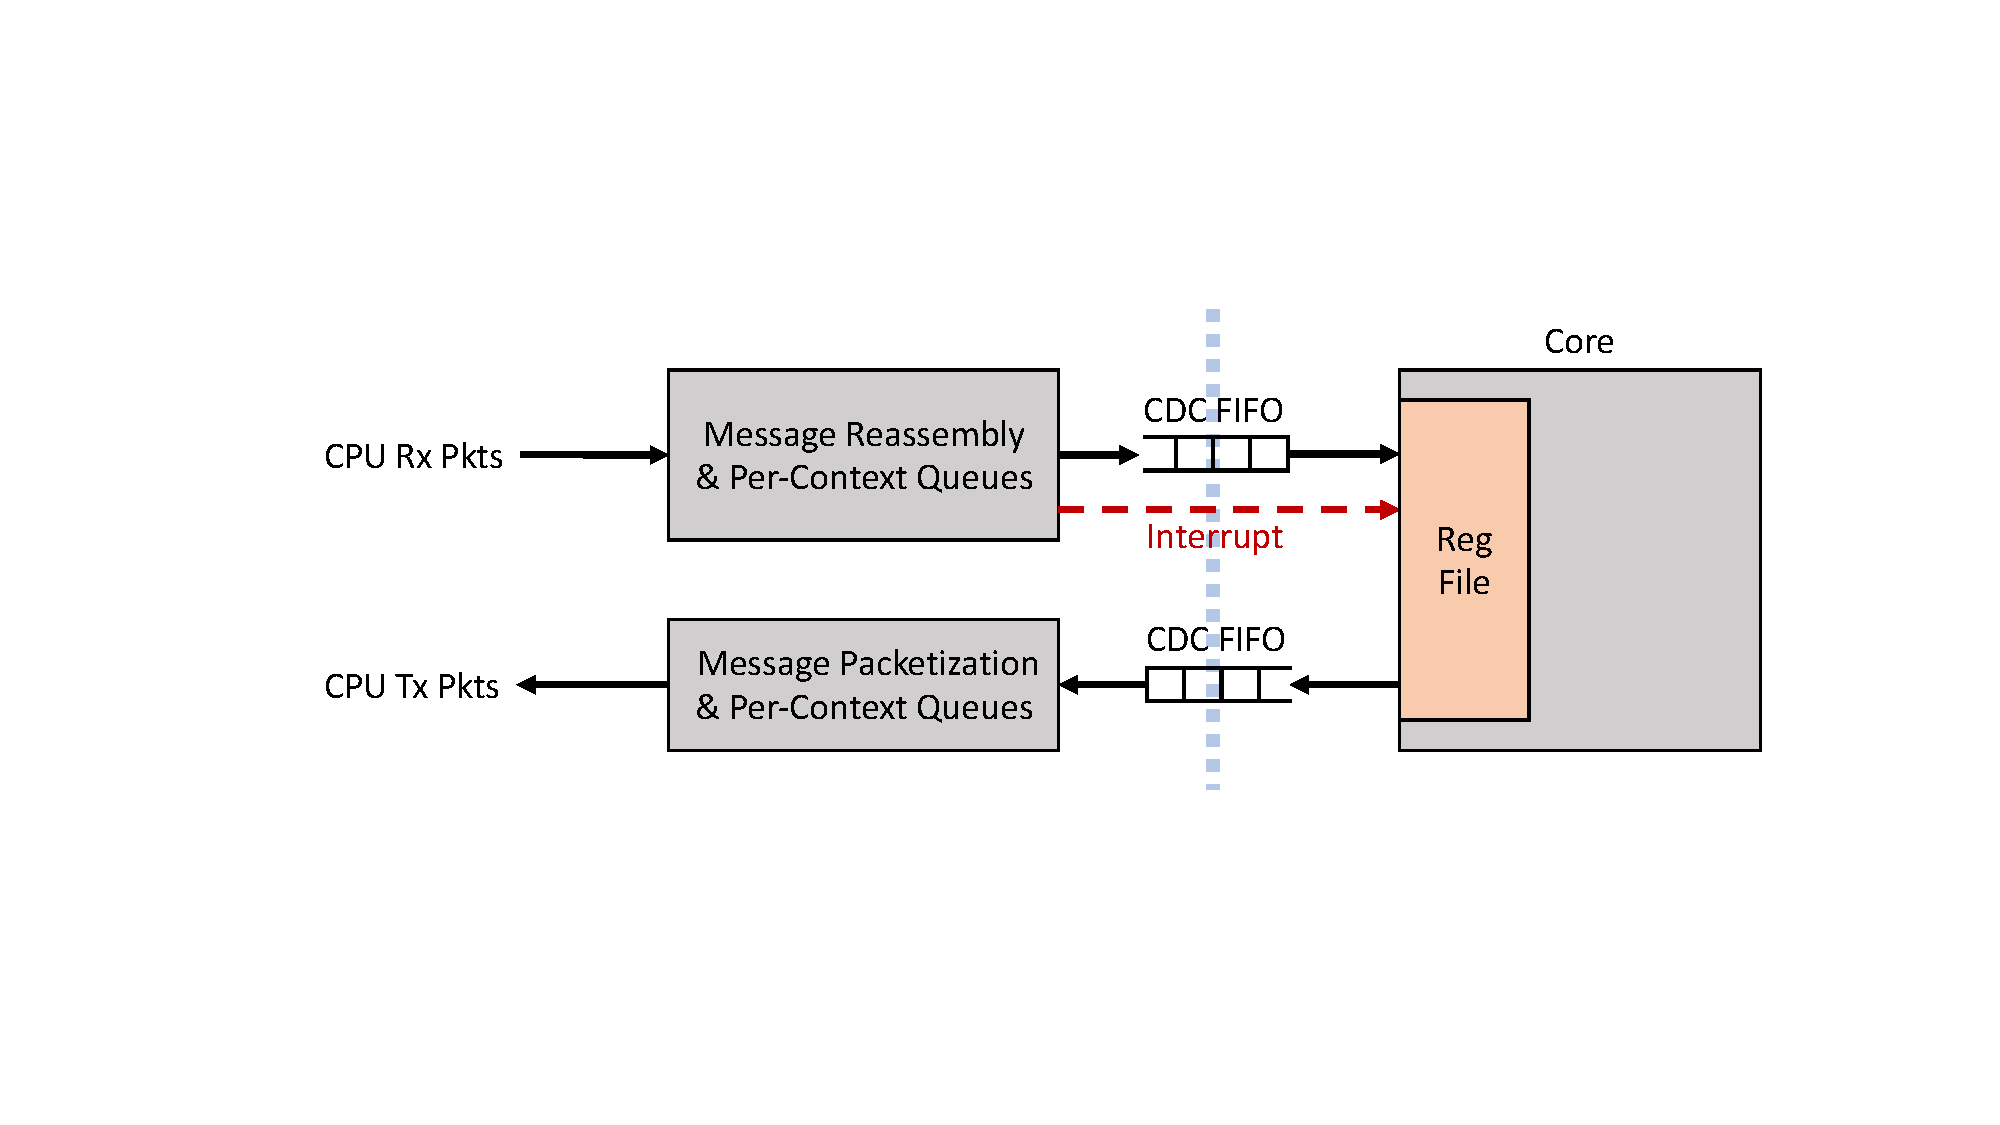
\includegraphics[width=\linewidth]{./figures/NIC-Core-Interface}
  \caption{Block diagram of the NanoPU's NIC-Core interface.}
  \label{fig:NIC-Core-Interface}
\end{figure}
\begin{itemize}
    \item The key component of the NanoPU's NIC-Core interface is its fast path directly into the CPU's register file. This is implemented using a simple FIFO interface between the NIC and the register file.
    \item We propose very minor modifications to the host CPU in order to support our fast path.
    \item We reserve two general purpose registers (GPRs), one for the head of the RX queue and one for the tail of the TX queue of the current context (i.e. application thread).
    \item The underlying hardware supports per-context TX and RX queues and only exposes the queues of the currently running context via the head/tail GPRs.
    \item As a result of the fact that the CPU pipeline and the NIC may run at different clock frequencies, we use simple clock-domain crossing FIFO queues between the per-context queues and the CPU pipeline.
    \item The NIC exposes a message interface to applications running on the core. This means that the hardware is responsible for performing message packetization and reassembly. Both of these are tasks that we will describe in more detail in our subsequent paper, which will include a description of the NanoPU transport protocol. In this paper, we will assume that all application messages fit in a single Ethernet packet. We expect that this will be sufficient to implement the vast majority of nanoservice applications.
    \item The NIC-Core interface also includes a few additional control status registers (CSRs) and memory-mapped registers, which are used to perform out-of-band configuration of the NIC, such as registering/deregistering context IDs with the NIC, supporting NIC-driven thread scheduling, and adding/removing PISA table entries.
    \item The first 8 bytes of every message sent and received by the application consists of a small application header.
    \item The application header indicates message length as well as the source IP address and context ID for received messages, or destination IP address and context ID for transmitted messages. This header allows the application to know when it has reached the end of a message. It also allows the NIC to know when the last byte of a message has been written to the TX queue by the application.
\end{itemize}

\subsection{Transport Termination in the NIC}
\begin{itemize}
    \item This section describes the hardware mechanisms in the NanoPU architecture that enable the NIC to terminate a low latency transport protocol such as Homa.
    \item We describe the hardware mechanisms, but the actual implementation and evaluation of a specific transport protocol is outside the scope of this paper and will be presented in a future paper.
    \item By terminating the transport protocol in hardware, the overhead required for applications to send/receive small messages is significantly reduced. It is very inefficient for software to deal with per-message timers, packet retransmissions, message reassembly and packetization, while hardware can implement this functionality much more efficiently.
    \item The key hardware components that enable the NIC to terminate a low latency transport protocol are as follows:
    \begin{itemize}
        \item An Event-driven PISA pipeline in the NIC data path. This programmable data-plane architecture enables us to process data-plane events in the background of data packet processing, that is, without affecting the rate at which data packets are processed. It does this by scheduling and aggregating memory accesses.
        \item A timer event generation module that is able to maintain $N$ timers (e.g. one per active message or one per active RPC). The timer module supports the following three operations per-timer: schedule (i.e. add a new time), reschedule (i.e. restart an existing timer), and cancel (i.e. remove the state associated with an existing timer). These timer events are processed in the background of data packet processing and are used to determine when a data packet retransmission must be sent or when a message has expired. All timers must be constrained to have the same period in order to make the hardware design scalable. We do not anticipate this to be a major limitation.
        \item In addition to data packet processing and timer event processing, the Event-driven PISA pipeline also supports background state clean up event processing, which is triggered either when: (1) message transmission / reception is complete, or (2) message transmission / reception has expired (i.e. timed out).
        \item A programmable packet generation module that can be programmed to generate acknowledgement and/or message completion packets.
        \item A packetization buffer that buffers messages sent from the CPU and generates packets that are subsequently processed by the Event-driven PISA pipeline before being transmitted. It also supports retransmitting data packets within a message.
        \item A message reassembly buffer that is able to reassemble potentially multi-packet messages with duplicate packets into a single message that is then delivered to the appropriate RX queue for the destination context.
        \item The transport header has the following fields:
        \begin{itemize}
            \item Source / destination context ID
            \item Message ID
            \item Message length
            \item Packet offset within the message
            \item Reserved bits for layering RPC request/response support on top of a one-way reliable message protocol
        \end{itemize}
    \end{itemize}
\end{itemize}

\subsection{The NanoKernel}
% \todo[inline]{Describe NanoKernel interaction with NIC. Describe nanoservice interaction with NanoKernel.}
\begin{itemize}
    \item One of the main goals of the NanoPU is to put as many cores in the network in the most cost effective way possible. Ideally, nanoservice application developers will be able to utilize enough cores to exploit all possible parallelism in their application, which could reach beyond millions of cores. Application parallelism could exceed the number of physical cores that are available. \chang{What do we mean by this last sentence? What's application parallelism? The total demands of applications for nanoservices?}
    \item Thus, NanoPU cores must be multiplexed very efficiently. We cannot rely on slow software-based scheduling mechanisms to schedule nanoservice threads. Instead, the NIC drives thread scheduling. The NIC keeps track of the highest priority context with messages to process and interrupts the CPU pipeline under two conditions:
    \begin{enumerate}
        \item A message arrives for a higher priority context than the one currently running on the core.
        \item The current context tells the NIC it is idle and the NIC sees that there is another context with messages to process.
    \end{enumerate}
    \item When the NIC interrupts the CPU pipeline it tells the NanoKernel scheduler which context to switch to. The NanoKernel thread scheduler simply performs a context switch to the context indicated by the NIC.
    \item When an application wants to perform network IO it issues a system call providing its desired context ID and priority. The privileged system call code will then ensure that the desired context ID is available and will register the context ID with the NIC along with the indicated priority level by performing writes to the appropriate CSRs. This operation is roughly equivalent to opening a socket on a modern operating system.
    \item Maybe also explain how the current implementation of the NanoKernel is different from a traditional operating system: applications are compiled into a single binary, shared address space, single privilege mode, etc.
    \item We require a minimal operating system to ensure that all code (and data) fits in on-chip SRAM.
\end{itemize}